\chapter{Kingdom of Fife}
{\entryfont \DndDropCapLine{F}or over a thousand years, the Kingdom of Fife stood as a beacon of strength and unity in the northern lands, founded by the legendary hero Dundax. From the city of Dundee, the royal bloodline ruled over a prosperous kingdom, its history intertwined with tales of valour, honour, and a long-forgotten prophecy that once foretold its fall. Now, on the eve of a grand wedding that promised to secure peace for generations, whispers of strange and unsettling phenomena began to emerge, though few took them seriously enough to cloud the celebrations.

}

\subsubsection*{The Birth of Dundax}
{\entryfont In the time before the founding of the grand city of Dundee, the lands of what would become the Kingdom of Fife were wild and untamed, roamed by warring clans and scattered settlements. It was during this era, in the year 20 B.D., that Dundax, the legendary hero, was born. Raised in the rugged hills of the north, Dundax was said to possess a strength and wisdom beyond his years, earning him the admiration of both chieftains and common folk alike. Tales of his feats spread quickly - how he single-handedly defended his village from raiders, how he tamed the wild beasts of the forests, and how he united rival clans through his courage and diplomacy.

Yet, it wasn't just his physical might that made Dundax a hero in the eyes of the people. A dreamer and a visionary, Dundax saw a future for Fife that transcended the tribal skirmishes of his time. He imagined a kingdom, one where peace could flourish and where his people could thrive under a united banner.}

\subsubsection*{The Founding of Dundee}
{\entryfont By the year 0 A.D., Dundax had grown into a man of great renown. It was in this year that he gathered his followers and founded the city of Dundee. From the city's grand walls, rising from the banks of the silvery Tay River, Dundax proclaimed the birth of the Kingdom of Fife - a land where unity and prosperity would reign.

Dundee itself was a marvel of its time. Surrounded by fertile lands and guarded by the natural barrier of the river, it became a beacon for traders and settlers from across the land. Under the wise rule of Dundax, the kingdom began to grow, with smaller settlements and clans swearing fealty to this new vision of peace and unity.

However, as Dundax stood on the heights of his newly founded city, a shadow loomed. Malyroth, a farseer from Anstruther, approached the city and spoke a prophecy that would echo through the ages: \textbf{"The prophecy is written. Dundee will fall!"} The words, though vague, struck fear into the hearts of those who heard them at the time. But as decades turned into centuries and the kingdom prospered without incident, the prophecy gradually faded into obscurity, remembered only by a select few scholars and keepers of ancient knowledge. For the vast majority of Fife's people, the prophecy of Dundee's fall became little more than an old myth, a forgotten relic of the past.}

\subsubsection*{The Founding of the Knights of Crail}
{\entryfont In the year 450 A.D., Prolon I, a visionary leader from Fyfdonia, a fertile region south of Dundee, founded the Order of the Knights of Crail. The knights quickly became known as a mystical and formidable force, renowned for their mastery of combat and their ability to ride giant, flying eagles. This gave them an unprecedented advantage in battle, and they earned a reputation as warriors who never opted out of a fight and were never defeated. The Knights of Crail became a symbol of Fyfdonia's strength and were revered not only for their prowess but for their mysterious and unwavering code of honor. Their presence in the region began to shape the political and military landscape of Fife.}

\subsubsection*{The Great Eagle War}
{\entryfont By the year 743 A.D., tensions between the principalities of Fyfdonia and Angus reached a breaking point, leading to the outbreak of the Great Eagle War. This conflict, named for the flying eagles of the Knights of Crail, saw Fyfdonia and Angus locked in bitter combat. Dundee, though officially neutral, was heavily affected by the conflict between its northern and southern neighbours.

The war raged for years, with both sides suffering significant losses. However, the might of the Knights of Crail, launching devastating aerial attacks from their eagles, proved overwhelming for Angus's ground forces. In a momentous agreement, the principalities of Angus and Fyfdonia were unified into a single kingdom, marking the birth of the Kingdom of Fife. The city of Dundee, with its strategic position and deep cultural significance, was declared the capital of this newly united realm. The Great Eagle War, though devastating, resulted in a lasting peace, with the once-warring regions now working together as a single kingdom.}

\subsubsection*{Angus McFife I and Iona McDougall}
{\entryfont In the year 992 A.D., a great celebration was planned in Dundee. \textbf{Angus McFife I}, Prince of Fife, was set to wed Iona McDougall, daughter of Ser Proletius, Grandmaster of the Knights of Crail. The marriage was not just a union of two noble houses, but a symbol of the continued unity and strength of the kingdom. It was said that the wedding would solidify the bond between the royal family and the Knights of Crail, ensuring peace and stability for generations to come.

The city of Dundee was alive with excitement. Streets were adorned with banners, musicians played in the marketplaces, and people from across the kingdom flocked to witness the royal wedding. Angus McFife I, a young man of great charm and valour, was beloved by the people. His bride-to-be, Iona, was known for her beauty and intellect, as well as her skill in diplomacy. Together, they seemed poised to usher the Kingdom of Fife into a new age of prosperity.

Yet, as the kingdom prepared for the joyous event, whispers began to surface of strange occurrences in the mountainous regions beyond the river Tay. There were scattered sightings of the kingdom's famed unicorns - creatures known for their}
\onecolumn
\begin{multicols}{2}
{\entryfont \noindent gentle nature and their gleaming, pure white coats - behaving in ways that unsettled those who saw them. Normally kind and serene, these unicorns were seen acting erratically - skittish and aggressive, fleeing from human contact. Stranger still were reports of unicorns with unusual, festering wounds that never seemed to heal, wounds that glowed with an eerie, unnatural light. Their once-brilliant fur had grown dull and dirty, as though corrupted by a dark and malevolent force.

The sightings, however, were few and far between, scattered across the remote and wild mountains where only the bravest of travellers ventured. As such, most dismissed these reports as exaggerations or simple superstitions. After all, the unicorns had always been a symbol of purity and light, cherished by the people of Fife for centuries. The odd behaviour of a few unicorns in distant lands seemed insignificant in the face of the grand wedding and the continued prosperity of the kingdom.

Still, for those who had encountered the strange unicorns first-hand, there was a growing sense of unease, though it remained unspoken. The royal family and the Knights of Crail quietly noted the reports but took no public action, choosing not to alarm the populace on the eve of such an important event.

The stage was set, not just for a royal wedding, but for a turning point in the history of Fife. As the city of Dundee prepared for joy, unseen forces began to stir in the shadows. And so, on the eve of Angus and Iona's wedding, the Kingdom of Fife stood on the precipice of its greatest trial. Would the kingdom survive the strange occurrences creeping from the mountains beyond the Tay, or was this the beginning of the end for the proud land that Dundax had founded so long ago? Only time would tell...}
\end{multicols}
\vspace*{-4em}\hfill\\
\phantomsection\addcontentsline{toc}{section}{Map of the Kingdom of Fife}
\noindent\begin{tikzpicture}[remember picture, overlay]%
		\node[opacity=1,inner sep=0pt,yshift=-3.35cm] at (current page.center){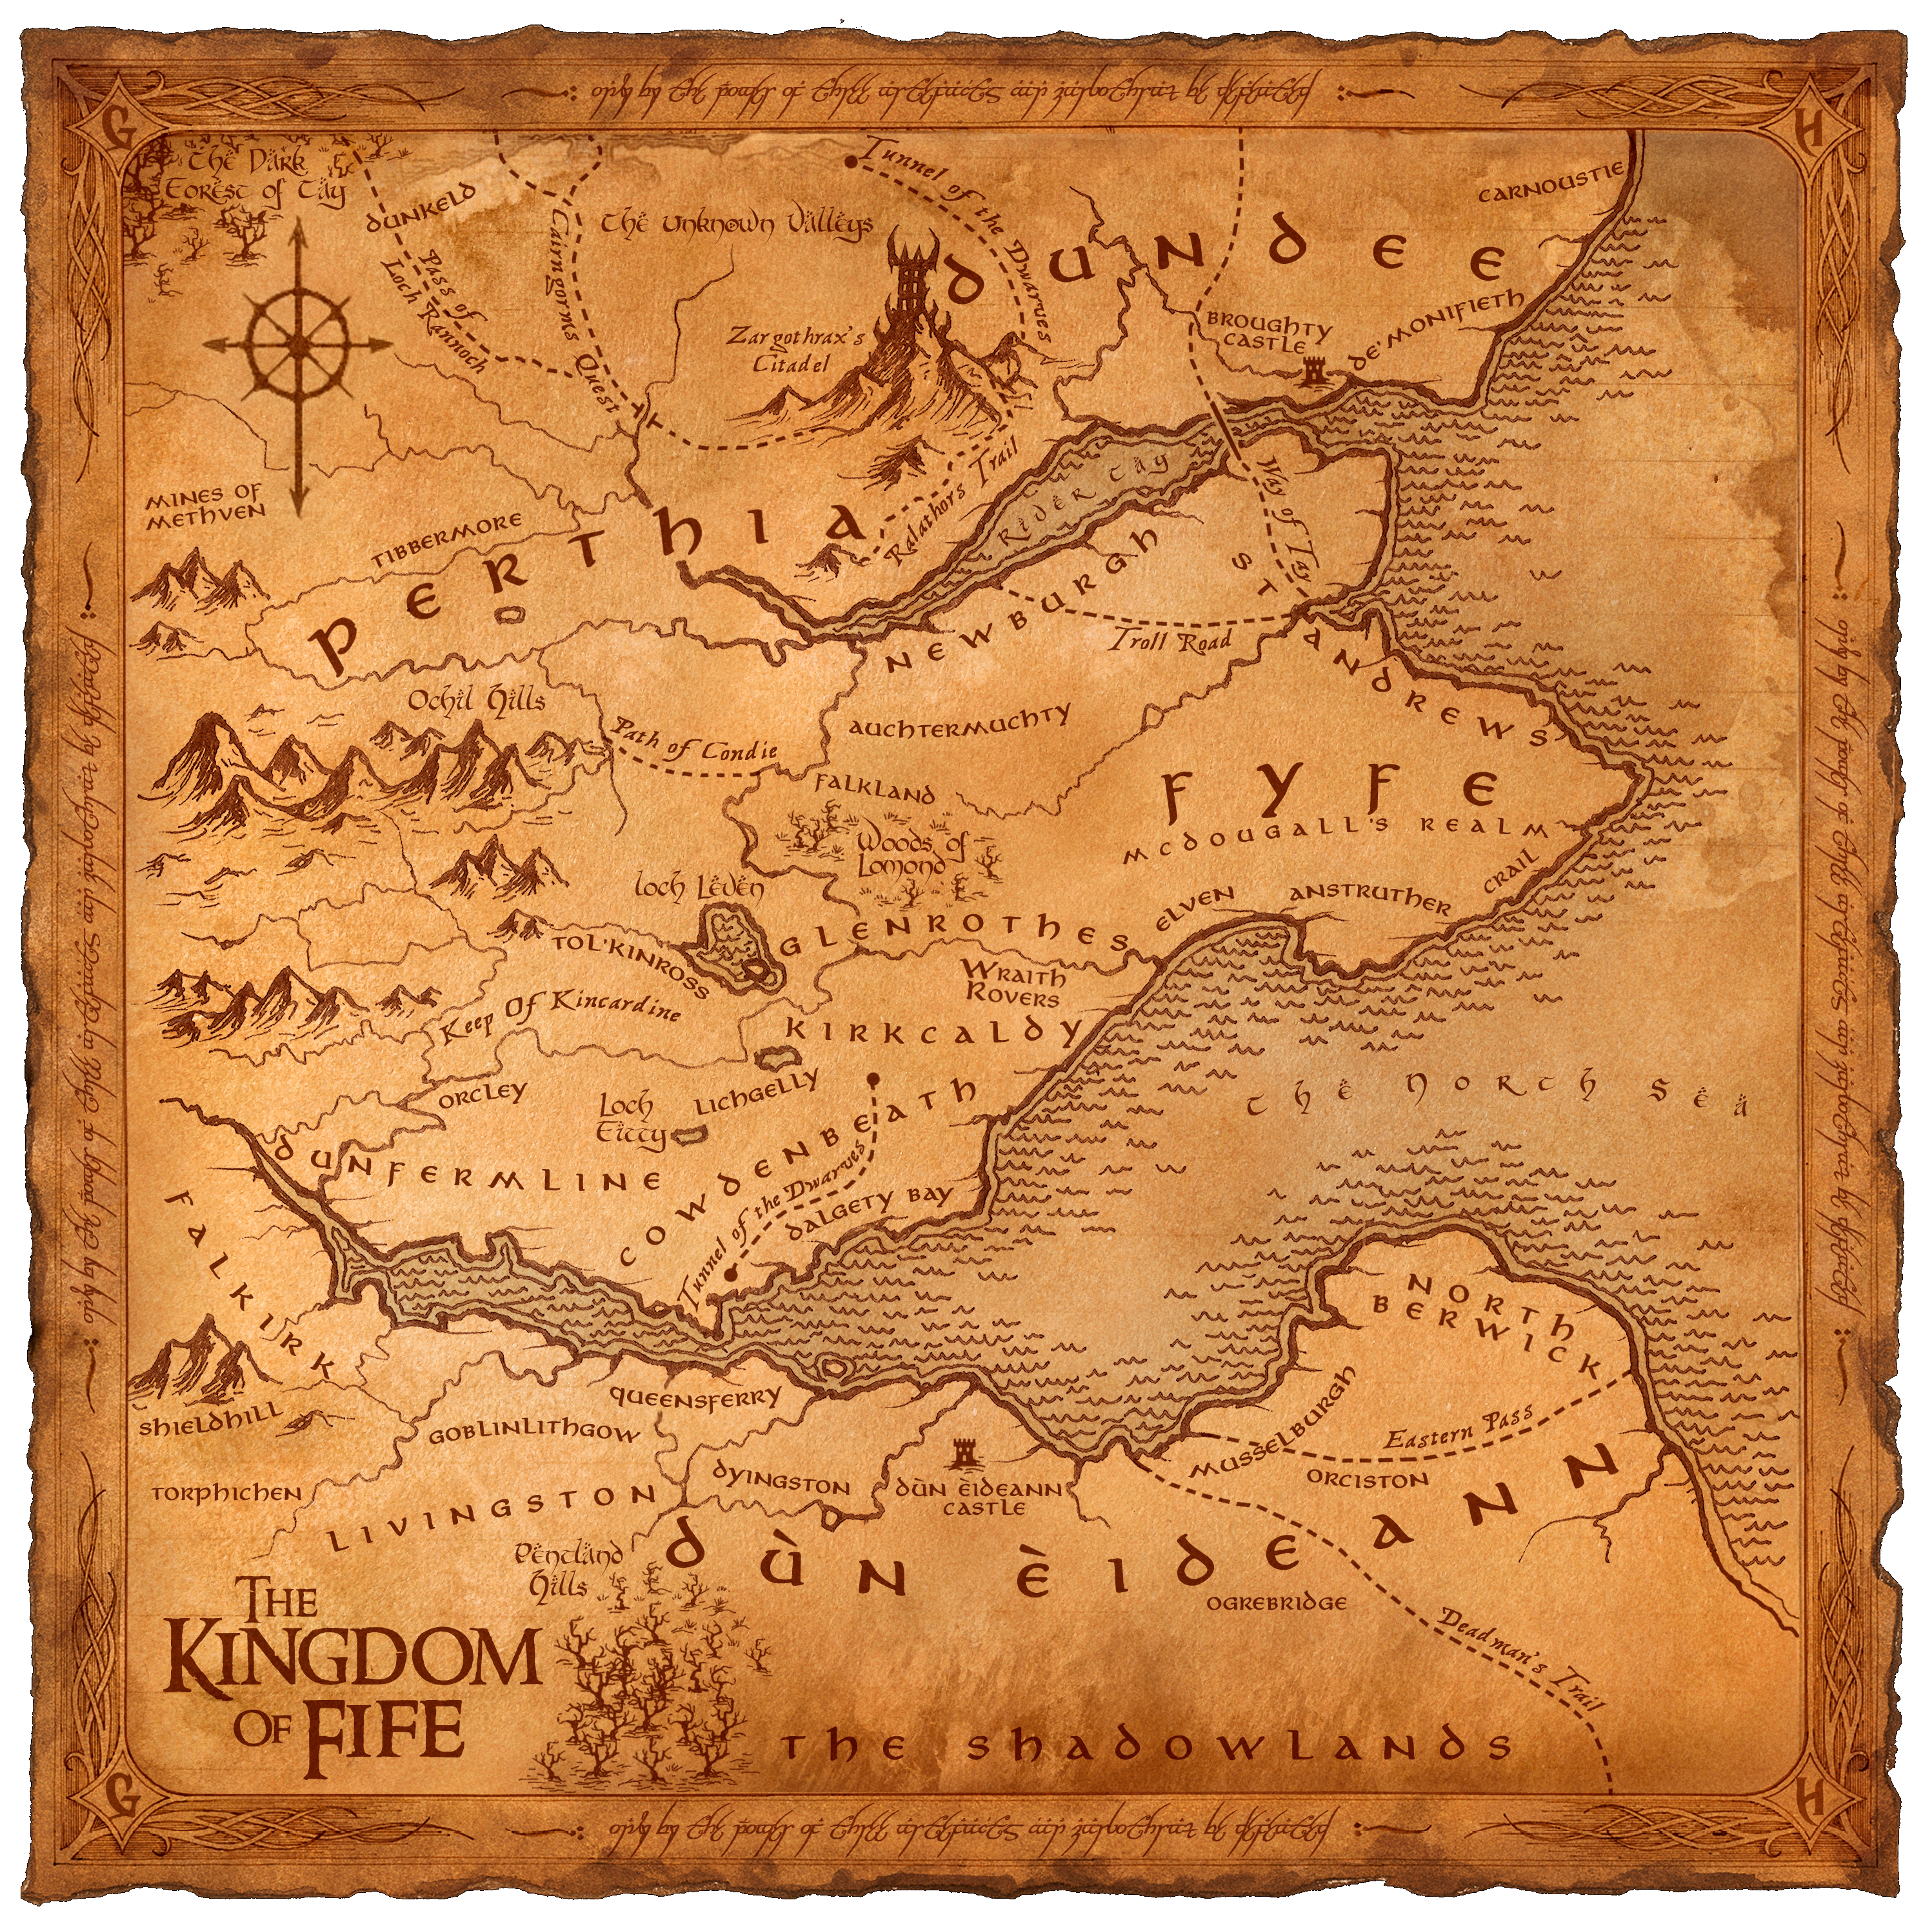
\includegraphics[width=\textwidth +8pt, keepaspectratio]{Kingdom_of_Fife_Map.png}};%
\end{tikzpicture}%
\twocolumn